\documentclass{article}
\usepackage{graphicx}
\graphicspath{{./Pictures/}}
\usepackage[table,xcdraw]{xcolor}
\usepackage{tabularx}

\title{Moj pierwszy rozdział}
\author{Dagmara Krenich}
\date{04.11.2022}
\begin{document}
\maketitle
\section{Matematyka}
Ciekawe wyrażenie matematyczne odkryte przez Einsteina:
\[ E = mc^ 2 \]\

\section{Oto moja lista: }

Moja lista kropkowana :
\begin{itemize}
    \item Tu mamy pierwszy element
    \item Tu mamy drugi element

\end{itemize}

Tu mamy listę numerowaną:
\begin{enumerate}
    \item Numerek pierwszy
    \item Numerek drugi

\end{enumerate}

\section{Zdjęcie}
oto jest zdjęcie: 

\includegraphics[width=\linewidth]{Pictures/Moje-male-pieski-Cover-410x290-zeszytowa-NB-f.jpg}
\breakpage
\section{Akapit}

\underline{\textbf{To jest mój przykład}} akapitu, który \underline{\textbf{chcę przedstawić}} w taki sposób: 
\emph{Ten akapit będzie napisany pod pewnym kątem}. \par \textbf{Ten natomiast jest wcięciem.} 
\\
Ten akapit jest napisany normalnie.
\\

`La \TeX {} to system przygotowania dokumentów i znaczników dokumentów
język. \LaTeX {} używa programu składu tekstu \TeX {} do formatowania
jego wyjście, a sam jest napisany w języku makr 
 \TeX {} . \LaTeX {} nie jest nazwą konkretnego (wykonywalnego) programu składu, ale
odnosi się do zestawu poleceń ( makr \TeX {} ), które tworzą znacznik
konwencje używane do składania dokumentów \LaTeX {} 

\section{Tabela}
\begin{tabularx}{0.8\textwidth} { 
  | >{\raggedright\arraybackslash}X 
  | >{\centering\arraybackslash}X 
  | >{\raggedleft\arraybackslash}X | }
 \hline
 pierwsza komórka & druga komórka & trzecia komórka \\
 \hline
 czwarta komórka  & piąta komórka & szósta komórka  \\
\hline
\end{tabularx}
\section{Odwołanie}
\begin { rysunek }[h!]
   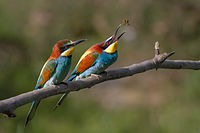
\includegraphics[skala=1.7]{Pictures/birds.jpg}
  \caption { Ptaki } 
  \label { rys:ptaki } 
\end { rysunek }
\end{document}